\chapter{Introducción}\label{cap:introduccion}

En este capítulo se introducirá el contexto en el que se ha desarrollado este TFG. Para ello, es necesario proporcionar definiciones y un resumen del estado del arte de las dos disciplinas en cuya intersección se encuentra el trabajo realizado: la robótica y las tecnologías web. 

\section{Robótica}

La robótica se puede definir como la técnica y la ciencia para el diseño, fabricación y operación de sistemas robóticos o robots. A su vez, también se puede considerar como la unión de la ingeniería mecánica, la electrónica, la informática y la inteligencia artificial.

Por otra parte, un robot se define como un sistema informático con sensores, actuadores y computador(es), que necesita ser programado para realizar tareas y que es sensible a la situación de su entorno.

\subsection{Estado del arte}

Desde los inicios de la robótica moderna, definida por Isaac Asimov en su libro \textit{I, Robot}, a mediados del XX, la robótica se ha expandido desde sus comienzos en las industrias con brazos robóticos hacia la conocida como robótica de servicios. Los robots de servicio que son definidos como aquellos que trabajan en lugares no industriales o de otra forma son aquellos capaces de realizar funciones en un rango mayor de entornos, que normalmente son cambiantes y no estructurados. 

Como se refleja en la definición de robot, todo sistema robótico está compuesto por tres componentes básicos: sensores, actuadores y computadores en los que se ejecutan distintos tipos de algoritmos que reciben información de los sensores y envían un comando a los actuadores para realizar la acción correspondiente.

En los últimos años, gracias a los avances en la capacidad de cómputo de los computadores, principalmente GPUs, y al exponencial progreso en las técnicas de inteligencia artificial, ha causado un aumento considerable en el número de sistemas que usan algoritmos basados en el aprendizaje automático, como redes neuronales o \textit{Reinforcement Learning}.

Un ejemplo de las áreas donde las aplicaciones robóticas han avanzado más en tiempo reciente son: 

\begin{itemize}
    \item \textbf{Agricultura:} los tractores autónomos, equipados con distintos accesorios como actuadores, sistemas de monitorización, localización y procesamiento de datos, son capaces de realizar tareas como el control de malas hierbas, la siembra o cosecha, sin o con mínima intervención humana. Este sector se espera que crezca notablemente durante los próximos años, aunque ya hay empresas que ofrecen estos servicios como Monarch, John Deere o Naio Technologies (\ref{fig:agricultura}).
    \begin{figure}[H]
        \centering
        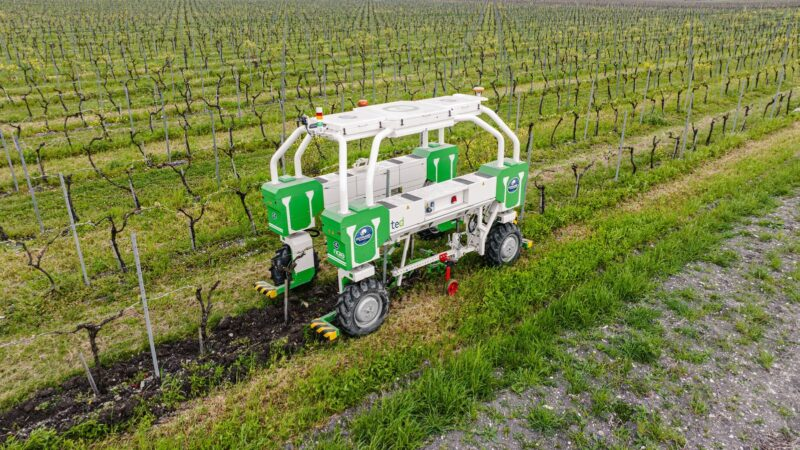
\includegraphics[width=0.4\textwidth]{figures/intro/agricultura.jpg}
        \caption{Robot de limpieza de viñedos de la empresa Naio Technologies}
        \label{fig:agricultura}
    \end{figure}

    \item \textbf{Conducción Autónoma:} los vehículos autónomos están equipados con sistemas avanzados de detección, procesamiento de datos y actuadores. Estos son capaces de navegar en el tráfico sin necesidad de intervención humana en la mayoría de escenarios, lo que los sitúa en el nivel 3 en la escala J3016. Su desarrollo tiene como objetivo mejorar la seguridad vial, aumentar la eficiencia del transporte y facilitar la movilidad de personas con diversidad funcional. Diversas empresas como Tesla, AutoX o Waymo (\ref{fig:autoX}) ya ofrecen servicios comerciales.
    \begin{figure}[H]
        \centering
        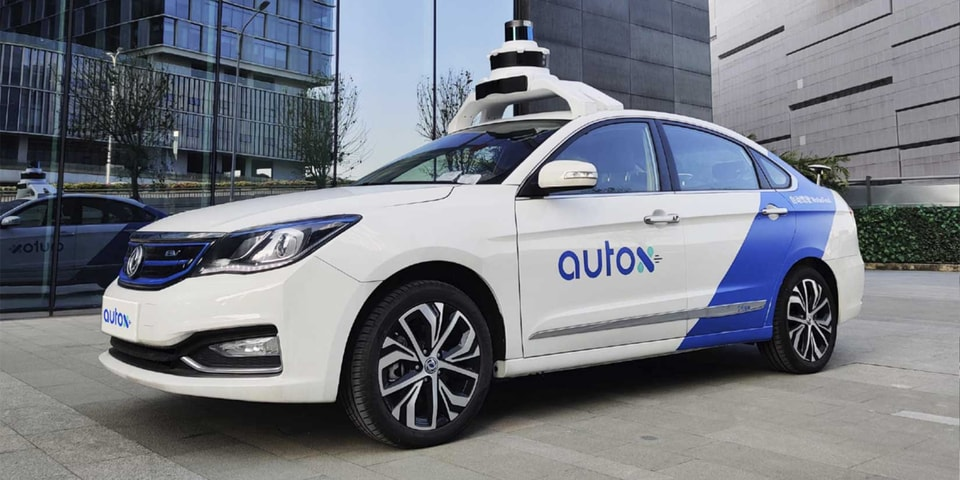
\includegraphics[width=0.4\textwidth]{figures/intro/autoX.jpg}
        \caption{Taxi autónomo de la empresa AutoX}
        \label{fig:autoX}
    \end{figure}

    % \item \textbf{Inspección y mantenimiento:} los robots, tanto drones como robots cuadrúpedos, realizan de forma más eficiente y segura la inspección de entornos de difícil acceso o de gran superficie. Están equipados de sensores que suelen ser cámaras o LIDARs y algoritmos que componen todos los datos tomados en un solo modelo para su posterior análisis que puede ser de forma automática o manual.  \ref{fig:inspección}
    % \begin{figure}[H]
    %     \centering
    %     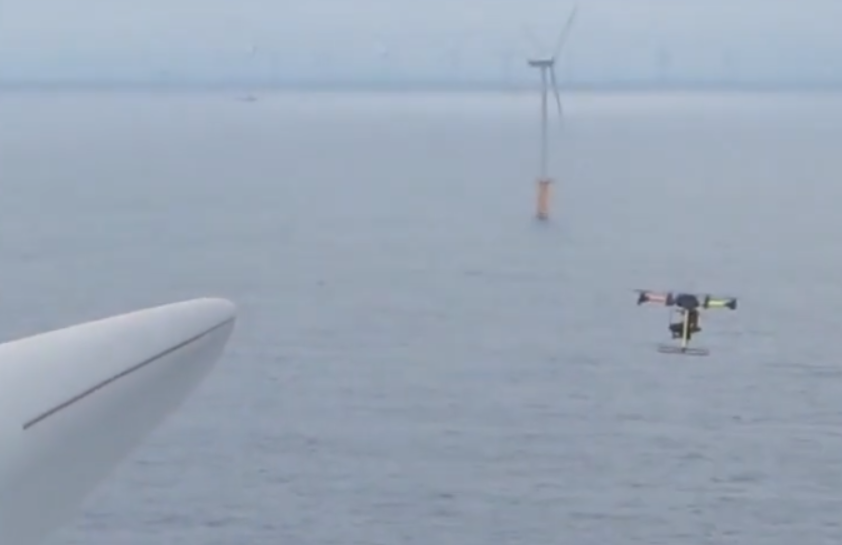
\includegraphics[width=0.6\textwidth]{figures/intro/drone.png}
    %     \caption{Robot de inspección de aerogeneradores de la empresa Helvetis}
    %     \label{fig:inspección}
    % \end{figure}

    \item \textbf{Logística:} los robots son más eficientes que los humanos a la hora de transportar las mercancías entre distintos puntos de las instalaciones, ya que son capaces de realizarlo de forma autónoma y constante durante un mayor periodo de tiempo. Estos están equipados con sistemas de navegación avanzados y con sensores destinados a disminuir la posibilidad de fallo. \ref{fig:almacenes}
    \begin{figure}[H]
        \centering
        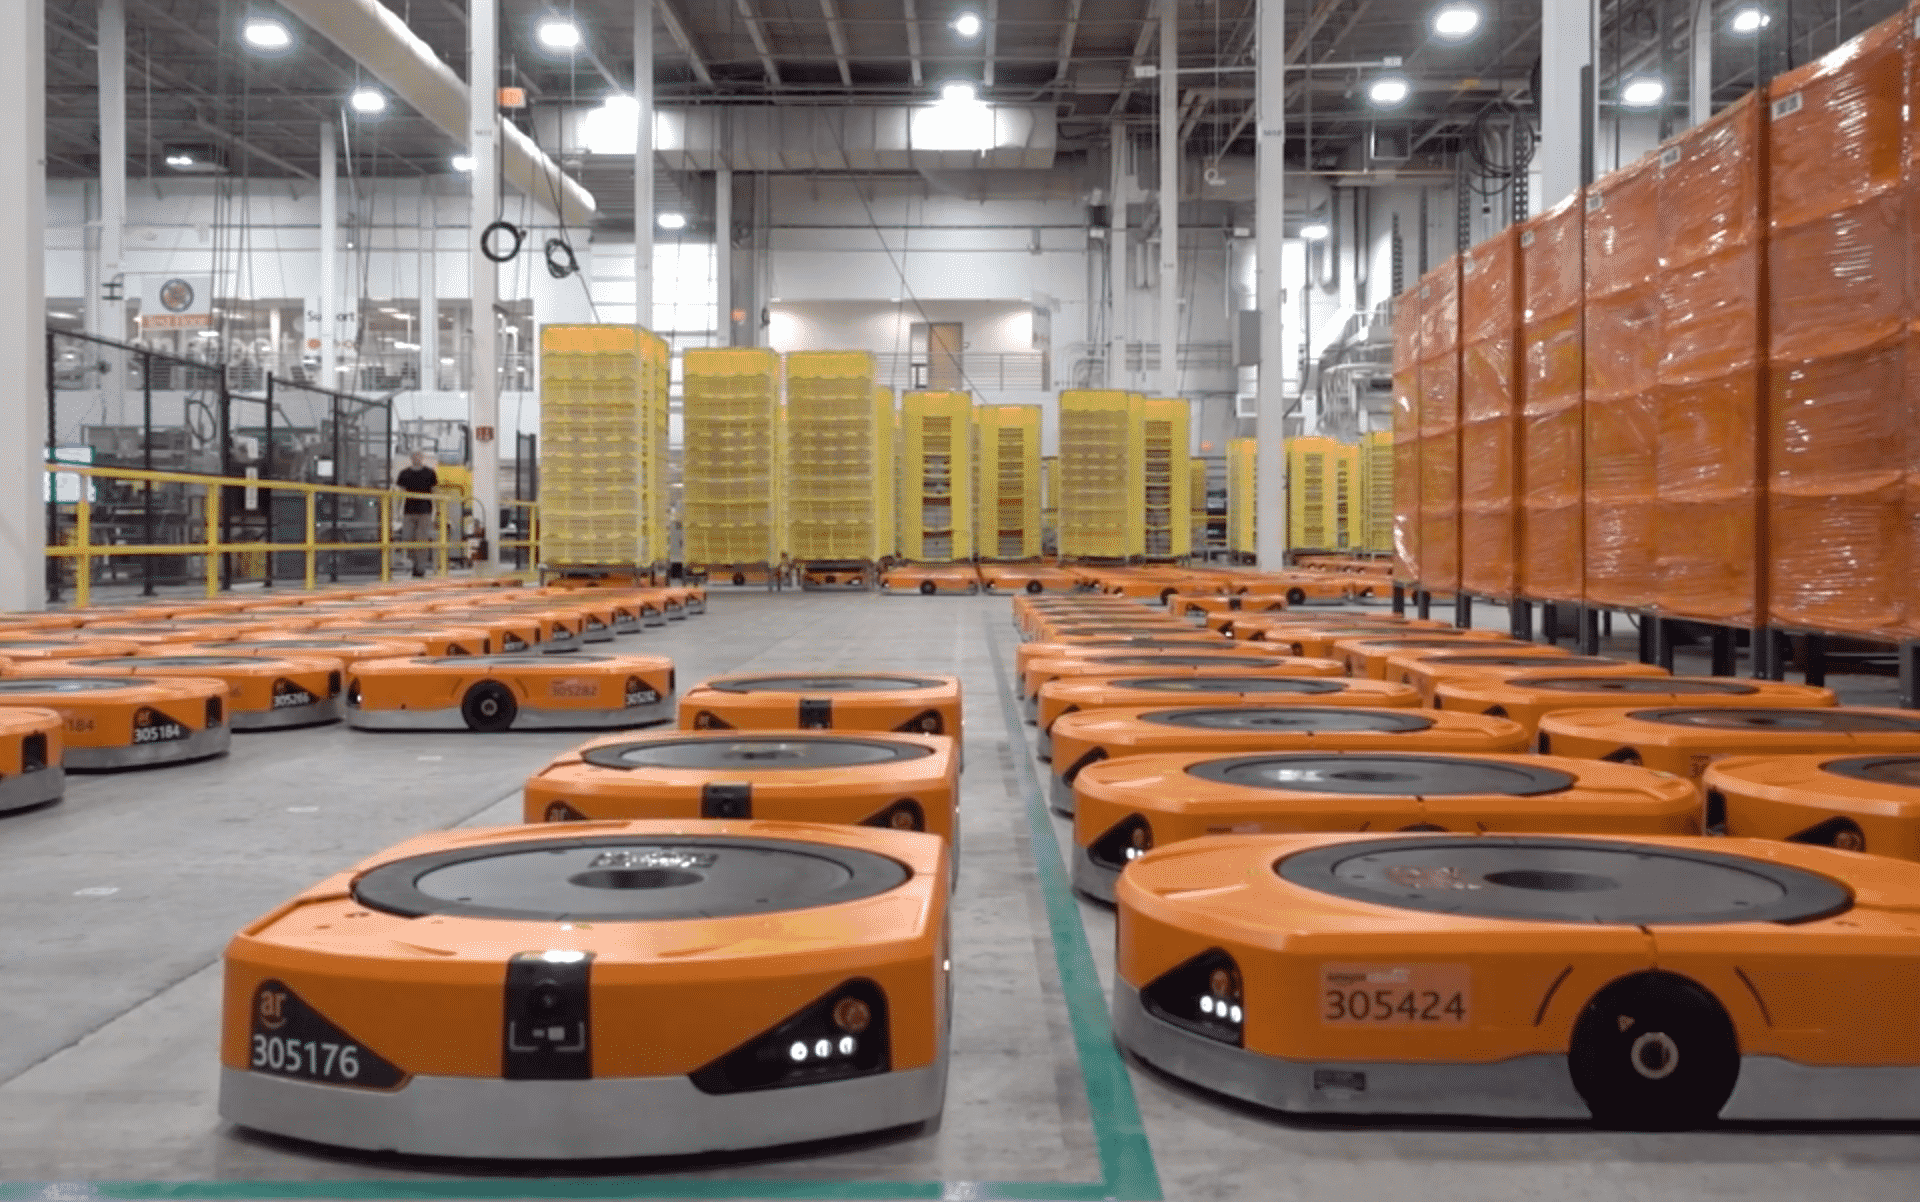
\includegraphics[width=0.4\textwidth]{figures/intro/amazon.png}
        \caption{Robots empleados en los almacenes de Amazon}
        \label{fig:almacenes}
    \end{figure}

    \item \textbf{Robots de Limpieza:} se encargan de la limpieza de diversos entornos, desde hogares hasta espacios públicos y oficinas, de forma autónoma usando algoritmos para planificar rutas de limpieza de manera eficiente. Incorporan sensores para detectar suciedad y obstáculos. \ref{fig:roomba}
    \begin{figure}[H]
        \centering
        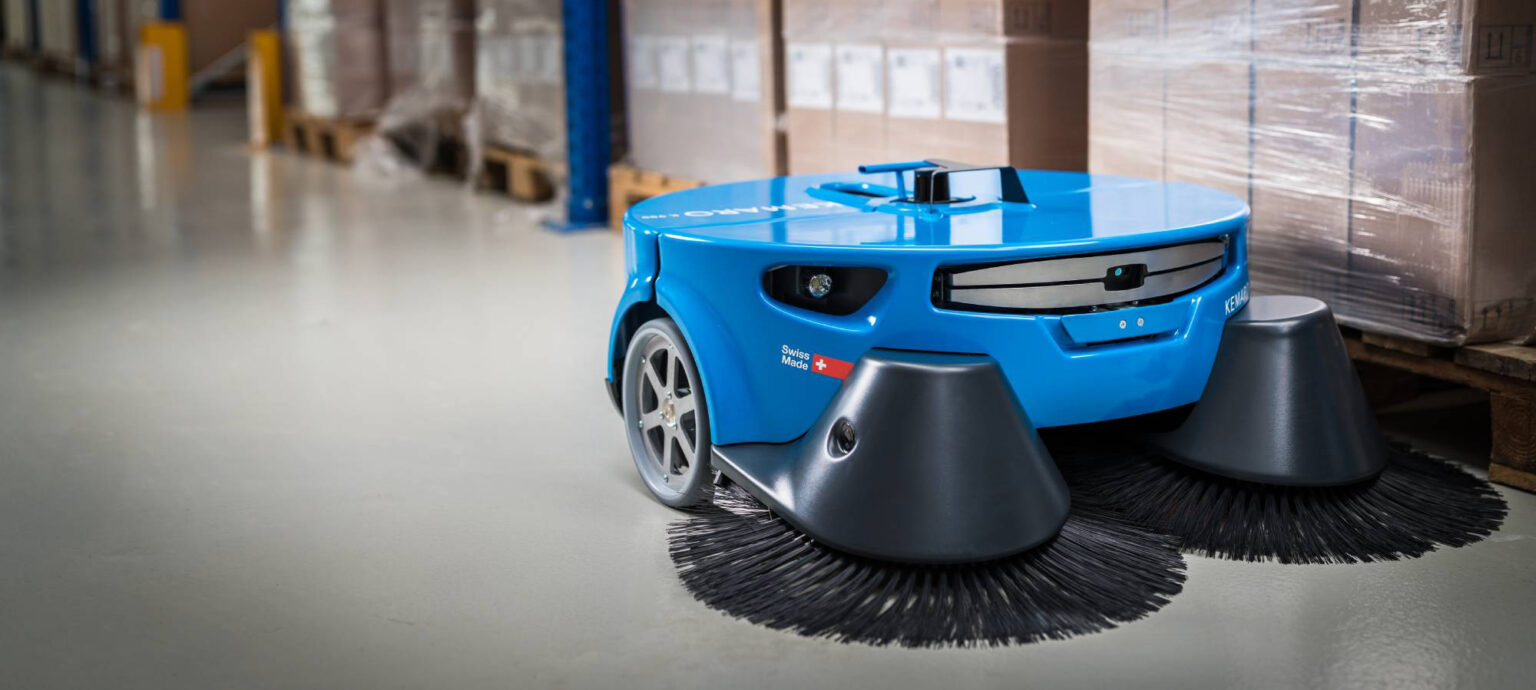
\includegraphics[width=0.5\textwidth]{figures/intro/vacuum.jpeg}
        \caption{Robot de limpieza industrial K900 de la empresa Kemaro}
        \label{fig:roomba}
    \end{figure}
    
\end{itemize}


\subsection{Desarrollo de aplicaciones robóticas}

Las aplicaciones robóticas han ido ganando complejidad para igualar a los avances en inteligencia artificial y en el desarrollo de componentes \textit{hardware}. La arquitectura software más utilizada actualmente en las aplicaciones robóticas es la de varios nodos distribuidos que ejecutan de forma paralela a distintos ritmos y que requieren de información variada para su funcionamiento. Este método es capaz de combinar las necesidades que requieren las aplicaciones robóticas, que son la reactividad para reaccionar e interaccionar con su entorno, y la toma de decisiones complejas y deliberadas. Con el fin de ayudar al desarrollo de aplicaciones robóticas han aparecido los \textit{middlewares} robóticos y los simuladores.

Los \textit{middlewares} robóticos ofrecen una abstracción del hardware y de las bibliotecas de comunicaciones para facilitar el desarrollo de aplicaciones. Estos \textit{middlewares} también tienen soporte para distintos simuladores. El más extendido en el mundo de la robótica, mayormente en la robótica de servicios, es ROS 2, que se explicará detalladamente en la sección \ref{ros_2}. ROS 2 soporta el uso de nodos distribuidos y su comunicación para desarrollar aplicaciones complejas.

\begin{figure}[H]
    \centering
    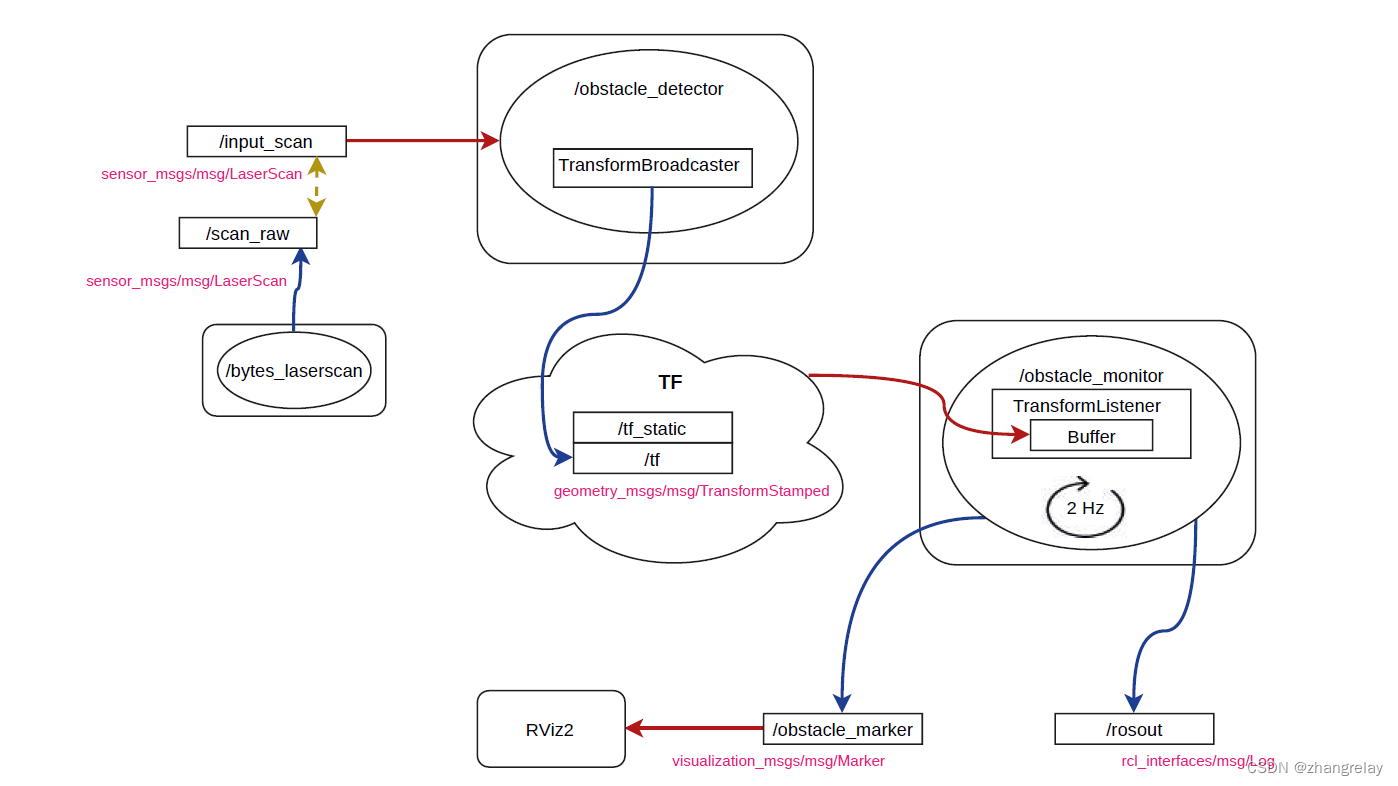
\includegraphics[width=0.7\textwidth]{figures/intro/c_graph.png}
    \caption{Grafo de nodos de una aplicación en ROS 2}
    \label{fig:ejemplo}
\end{figure}

Los simuladores permiten reproducir entornos físicos realistas para la depuración y ejecución de aplicaciones robóticas sin el riesgo de dañar equipos reales. Para ello, los simuladores tienen la capacidad de replicar distintos elementos físicos, como la gravedad, la colisión de objetos, la fricción, la luminosidad, etc. y ofrecen varios sensores y actuadores para su uso desde las aplicaciones robóticas. Todos estos elementos y parámetros son configurables, lo que permite simular de manera más detallada los diferentes mundos. Uno de los simuladores más utilizados es Gazebo (sección \ref{gazebo}), que cuenta con integración total con ROS 2.

\begin{figure}[H]
    \centering
    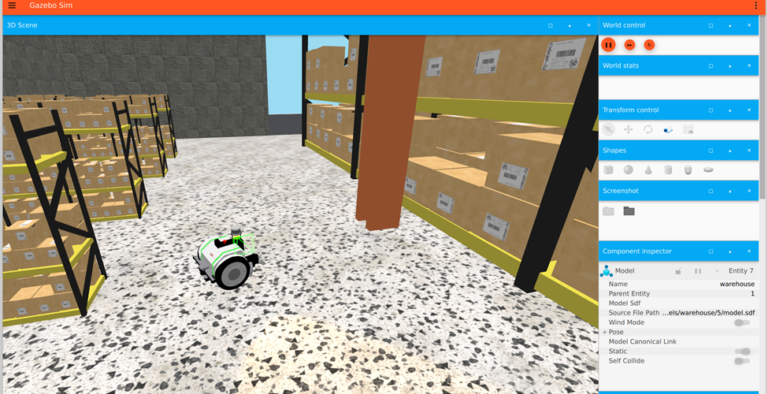
\includegraphics[width=0.6\textwidth]{figures/intro/gazebo.png}
    \caption{Entorno simulado en Gazebo}
    \label{fig:ejemplo}
\end{figure}

\subsection{Paradigmas de las aplicaciones robóticas}

Los componentes usados en las aplicaciones robóticas tienen funciones heterogéneas, pero pueden ser normalmente clasificados en tres tipos de componentes: 

\begin{itemize}
    \item \textbf{Componentes reactivos:} proporcionan una respuesta rápida ante cambios en el entorno. Están basados en el principio de estímulo-respuesta, lo que permite al robot actuar de forma rápida ante cambios no previsibles, sin necesidad de usar algoritmos de planificación de mayor complejidad. Habitualmente estos componentes realizan tareas que se deben ejecutar de forma inmediata y con alta frecuencia, como esquivar obstáculos o seguir una ruta. 

    \item \textbf{Componentes deliberativos:} realizan tareas complejas que requieren de la deliberación previa de múltiples factores y consecuencias. Permiten la toma de decisiones basadas en modelos internos del mundo, planificación a largo plazo de acciones complejas o la resolución autónoma de problemas. Se encargan de un abanico de acciones más amplio que los componentes reactivos, como la toma de decisiones, la navegación por entornos no conocidos o la coordinación de movimientos de brazos robóticos. Habitualmente estos componentes se ejecutan con una frecuencia menor y generan planes que ejecutarán los componentes reactivos.

    \item \textbf{Componentes de gestión de la ejecución:} proporcionan una forma de organizar y coordinar las acciones del robot, usando distintos estados. Hay de distintos tipos, pero los dos más usados son las FSM o máquinas de estado finito y los árboles de comportamiento. Las FSM permiten controlar la aplicación robótica dividiendo el comportamiento del robot en un número finito de estados, cuyas transiciones están definidas por un conjunto de reglas claras y deterministas. Por otra parte, los árboles de comportamiento proporcionan una abstracción de mayor nivel, lo que permite crear comportamientos más complejos y reutilizables. Estos últimos son los que más fuerza están ganando estos últimos años, ya que proporcionan una mayor sencillez de uso a la vez que permiten desarrollar aplicaciones más complejas, y también poseen de un mayor número de herramientas para facilitar su uso. Además estos facilitan la expansión de la aplicación.

\end{itemize}

\section{Tecnologías web}

\subsection{Estado del arte}

Las tecnologías web han sufrido una evolución exponencial en la última década, mejorando la experiencia de los usuarios y haciendo más eficientes, versátiles y accesibles las aplicaciones web. En el origen de Internet, las páginas web eran únicamente estáticas, creadas con HTML básico. Con el paso de los años se introdujo CSS, que permitió personalizar su estética, y JavaScript, que permitía conseguir interactividad en las páginas web. Esta última introducción conllevó la creación de diferentes \textit{frameworks} para la mejora del dinamismo y reactividad de las aplicaciones web, siguiendo cada uno de estos distintos paradigmas para su consecución. Los más usados hoy en día son React, Node.js, jQuery y Next.js.

\begin{figure}[H]
    \centering
    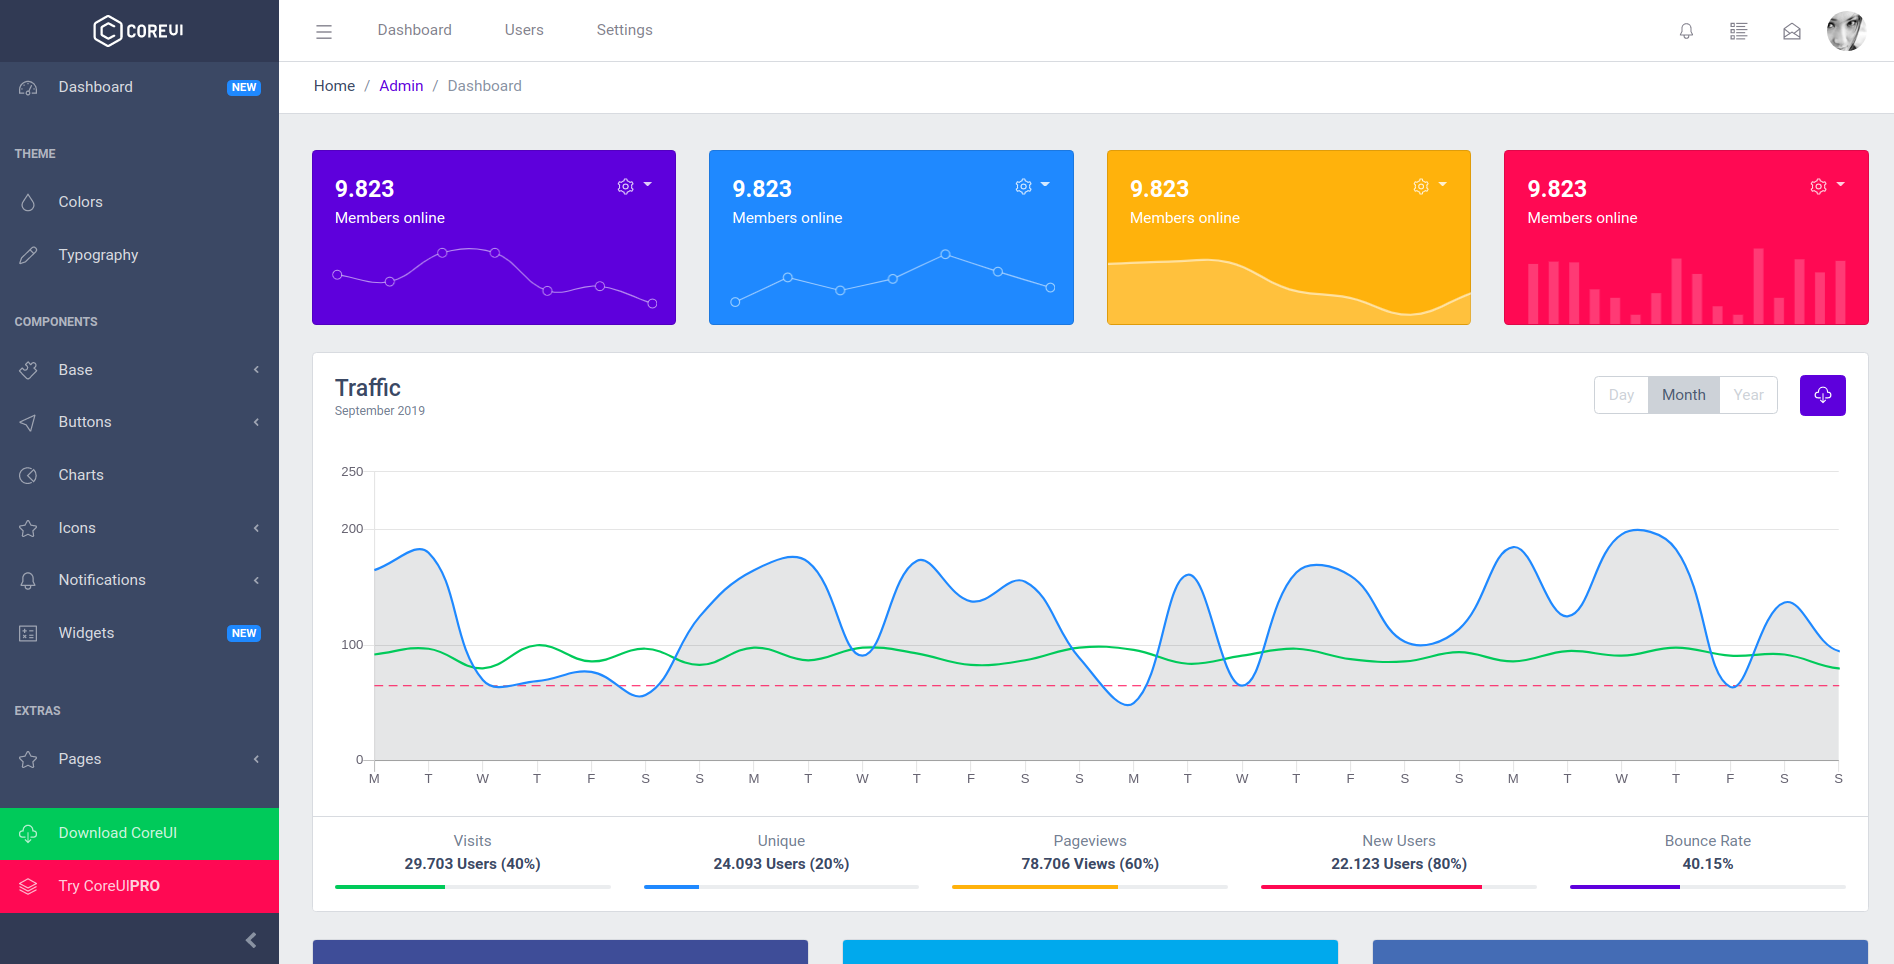
\includegraphics[width=0.6\textwidth]{figures/intro/react-ex.png}
    \caption{Interfaz creada con React}
    \label{fig:ejemplo}
\end{figure}

Por otra parte, también han evolucionado las tecnologías de bases de datos para satisfacer las necesidades de estas nuevas aplicaciones web. Las más populares son actualmente MySQL, PostgreSQL y MongoDB.

Algunos ejemplos de aplicaciones web modernas son:

\begin{itemize}
    \item \textbf{Plataformas de comercio electrónico}: estas permiten a los usuarios buscar, comparar y comprar productos con facilidad desde sus hogares. Utilizan tecnologías web avanzadas para ofrecer interfaces intuitivas y adecuadas al dispositivo de uso, así como procesos de pago seguros.

    \item \textbf{Aplicaciones de visualización de vídeos}: son aplicaciones web con elementos altamente reactivos, diseñada para transmitir contenido de video y audio a usuarios en todo el mundo. Estas utilizan tecnologías como WebRTC para proveer comunicación en tiempo real esencial para las videollamadas o el \textit{streaming}. 

\end{itemize}

\subsection{Plataformas web para programar}

En cuanto al ámbito de la programación, este también ha sufrido un gran auge en estos últimos años con la aparición de infinidad de plataformas o web IDEs creados para la educación o para el desarrollo profesional. Un par de ejemplos son las siguientes plataformas: 

\begin{itemize}

    \item \textbf{GitHub Codespaces\footnote{\url{https://github.com/features/codespaces}}}: ofrece un IDE donde los usuarios pueden escribir y desarrollar código en un entorno seguro integrado con GitHub. También permite compartir y probar código sin necesidad de configurar un entorno de desarrollo local.

    \item \textbf{Arduino Web IDE\footnote{\url{https://app.arduino.cc/}}}: permite desarrollar y cargar programas (\textit{sketches}) a placas Arduino directamente desde el navegador. Esta plataforma proporciona un IDE completo con todas las capacidades del IDE nativo como soporte para la edición de código, gestión de bibliotecas y acceso a una amplia gama de ejemplos.
    
\end{itemize}

\section{Plataformas web para la programación de aplicaciones robóticas}

La mezcla entre las tecnologías mencionadas anteriormente y la robótica da lugar a la aparición de plataformas web destinadas a la programación de aplicaciones robóticas desde el navegador. Para esto deben proporcionar adicionalmente un entorno para la simulación de la aplicación, algo que conlleva una mayor complejidad que la ejecución de código en los web IDE tradicionales. Estas plataformas se pueden dividir en dos dependiendo de la audiencia a la que vayan dirigidas:

\subsection{Plataformas educativas}

Aquellas enfocadas en el aprendizaje del desarrollo de aplicaciones robóticas o de conceptos relacionados con este ámbito. Las más conocidas a nivel internacional son: 

\begin{itemize}
    \item \textbf{TheConstruct\footnote{\url{https://app.theconstructsim.com/login/}}:} ofrece una amplia gama de cursos y simulaciones para aprender a programar robots usando ROS. La plataforma utiliza un IDE web y simuladores que corren en la nube, permitiendo a los usuarios desarrollar y probar sus aplicaciones y soluciones sobre robots simulados. Sus cursos abarcan todo tipo de niveles, cubriendo temas como la navegación, manipulación y percepción en entornos realistas. Figura \ref{fig:theconstruct}.

    \begin{figure}[H]
        \centering
        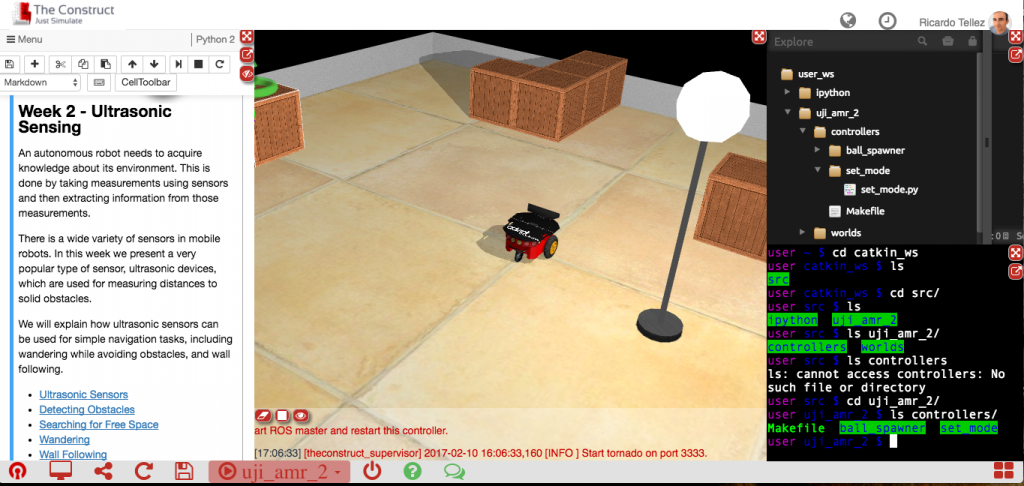
\includegraphics[width=0.7\textwidth]{figures/intro/theconstruct.png}
        \caption{Apariencia de TheConstruct}
        \label{fig:theconstruct}
    \end{figure}

    \item \textbf{Riders.ai\footnote{\url{https://riders.ai/en}}:} permite a los usuarios participar en competiciones de programación de robots, donde pueden medir sus habilidades contra las de otros programadores. A través de su IDE web, los participantes tienen la oportunidad de escribir, probar y optimizar su código en simulaciones que replican desafíos de robótica del mundo real. 
\end{itemize}

\subsection{Plataformas profesionales}

Estas tienen como propósito la programación y despliegue de soluciones robóticas en entornos de producción, ofreciendo una mayor gama de algoritmos y herramientas vanguardistas, dotando a la aplicación robótica de más complejidad y robustez que sus contrapartes educativas. Las dos plataformas más conocidas son:

\begin{itemize}
    \item \textbf{MoveitPro\footnote{\url{https://picknik.ai/pro/}}:} desarrollada por PickNik se centra en la programación de brazos robóticos en entornos no estructurados. Emplea árboles de comportamientos para la gestión de la ejecución de la aplicación, proporciona bloques predefinidos para tareas de planificación y percepción, entre otras funcionalidades como el uso de un simulador altamente realista (actúa como un gemelo digital) para facilitar la transición al brazo real. Está construido sobre la librería \textit{MoveIt}, estándar en la comunidad ROS 2 para la programación de brazos robóticos. 
    \item \textbf{Flowstate\footnote{\url{https://www.intrinsic.ai/flowstate/}}:} desarrollado por Intrinsic, una empresa propiedad de Google, y tiene como objetivo permitir la programación de aplicaciones industriales completas mediante un lenguaje de programación visual basado en bloques. Proporciona bibliotecas de bloques para tareas complejas y además, da a los usuarios la capacidad de expandirlas o crear las suyas propias. Por último, ofrece un entorno de simulación especializado, basado en ROS 2 y Gazebo.
    \item \textbf{Asimovo\footnote{\url{https://asimovo.com/}}:} plataforma de desarrollo de aplicaciones robóticas enfocadas en la robótica de servicio y proporciona una extensa colección de herramientas necesarias para el desarrollo de estas. Además, posee una \textit{biblioteca} de robots y de entornos de simulación. Figura \ref{fig:asimovo}.
    \begin{figure}[H]
        \centering
        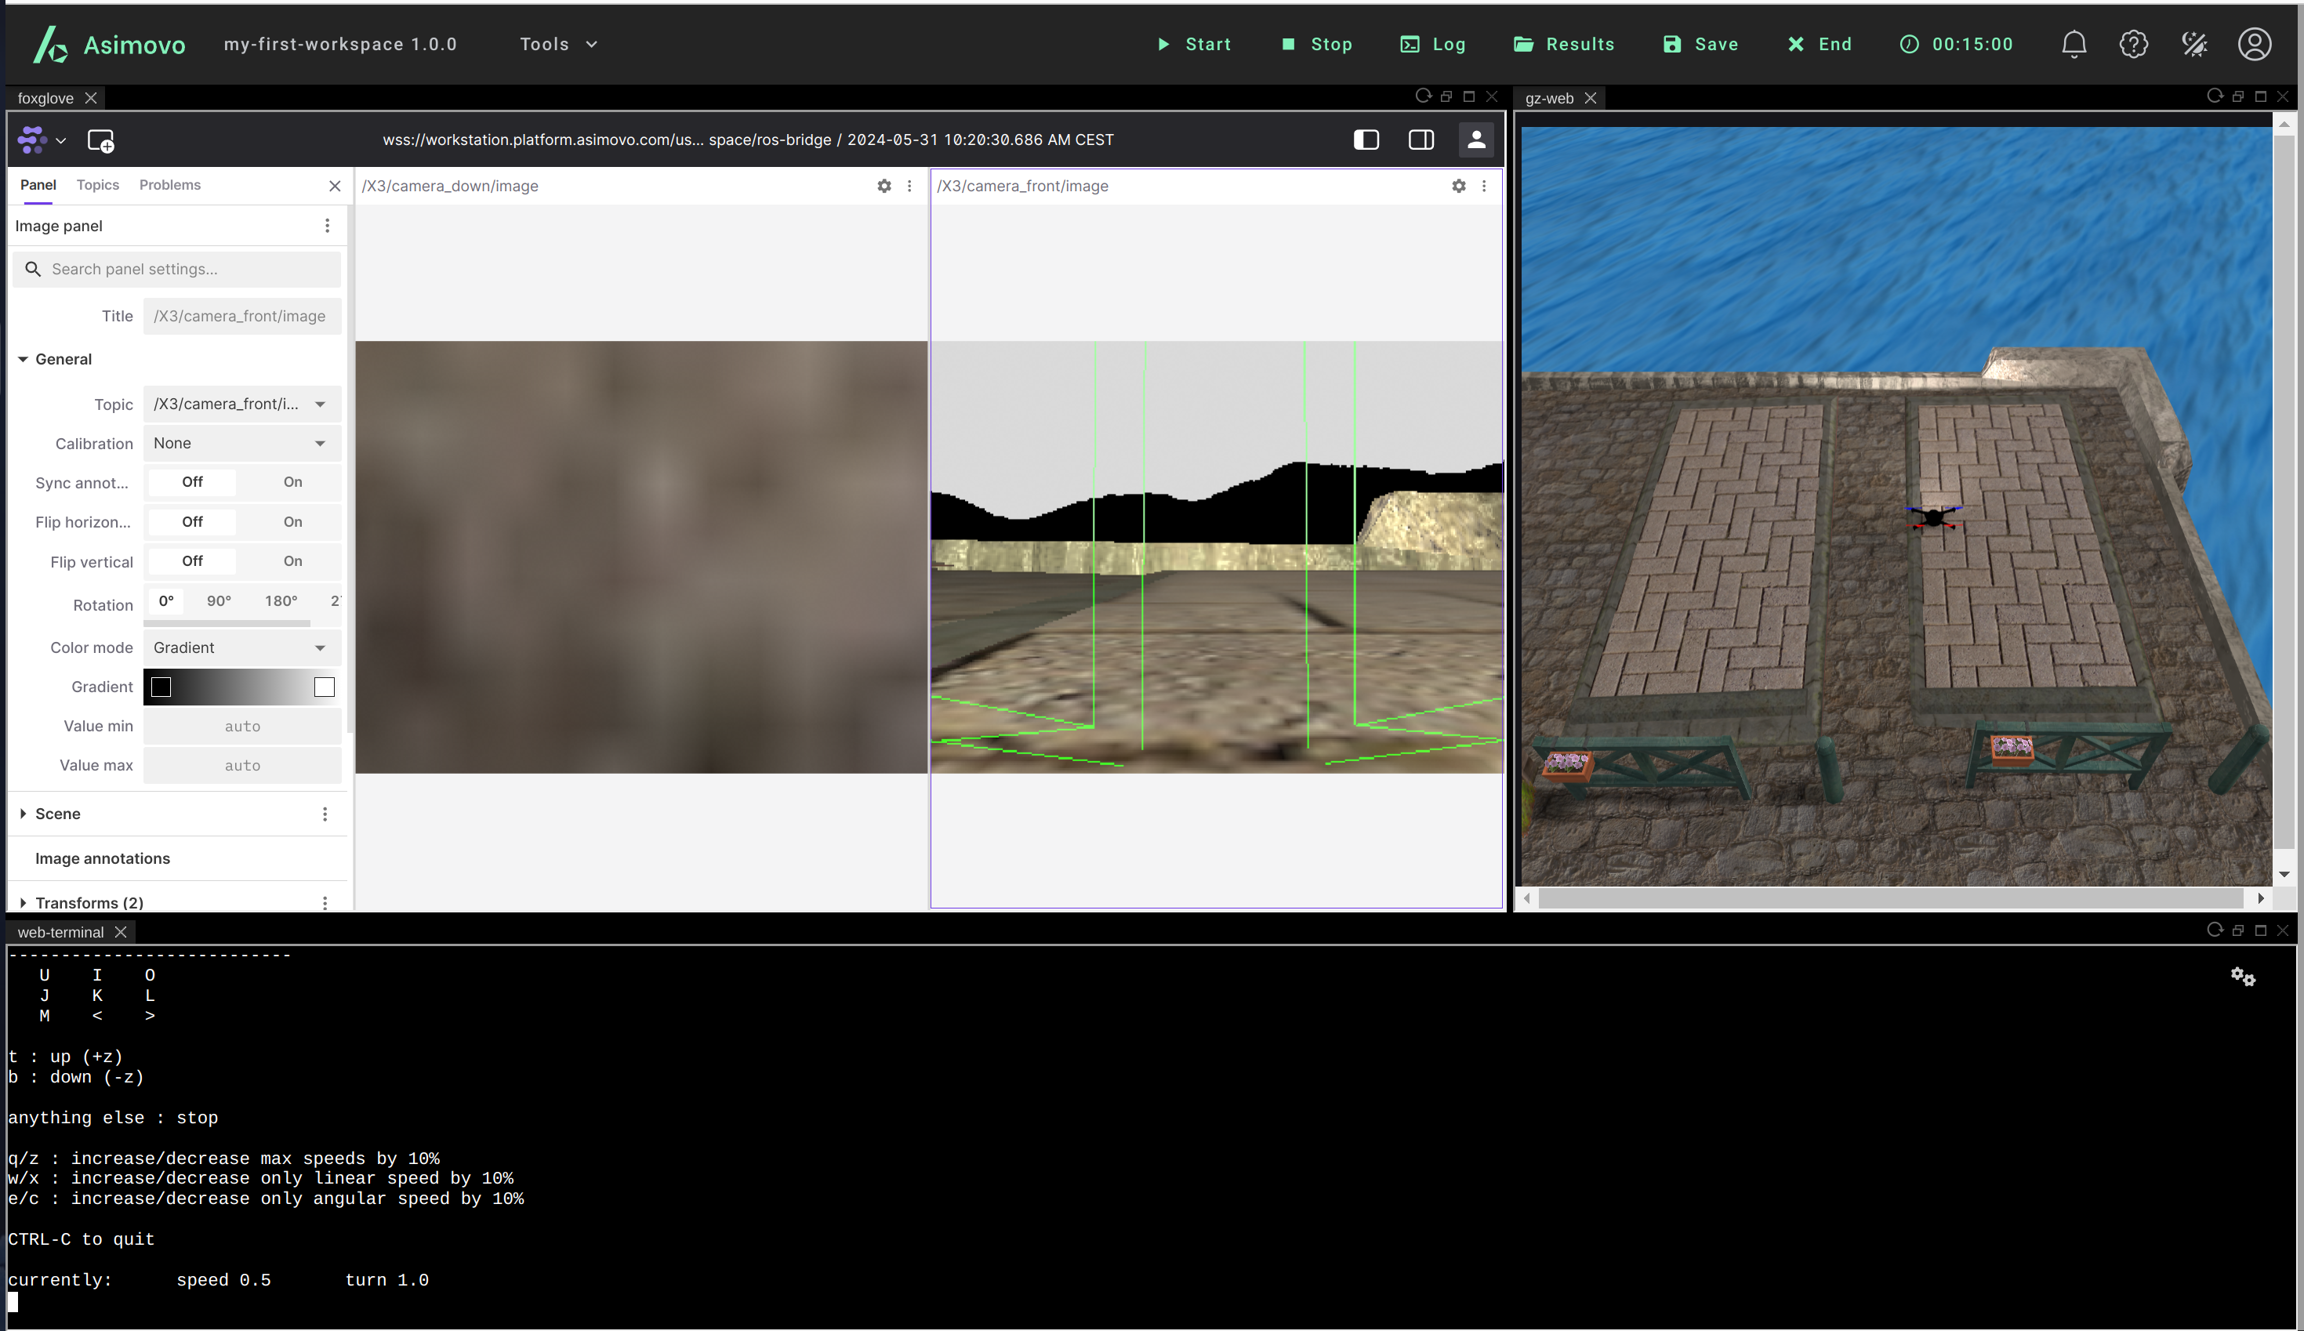
\includegraphics[width=0.7\textwidth]{figures/intro/asimovo.png}
        \caption{Apariencia de Asimovo}
        \label{fig:asimovo}
    \end{figure}
\end{itemize}

El objetivo principal de este TFG ha sido la mejora de BT Studio, una plataforma \textit{open source} que permite 
la programación de aplicaciones robóticas basadas en árboles de comportamiento desde un navegador web. 

